\chapter{}

\section{Enunciado}

Dado un autómata con pila configurado para acabar por el criterio de pila vacía, modificarlo para que funcione con el criterio de estados finales.

\section{Solución}

Vamos a generar el autómata mencionado en el enunciado:

\begin{figure}[h!]
\begin{center}
	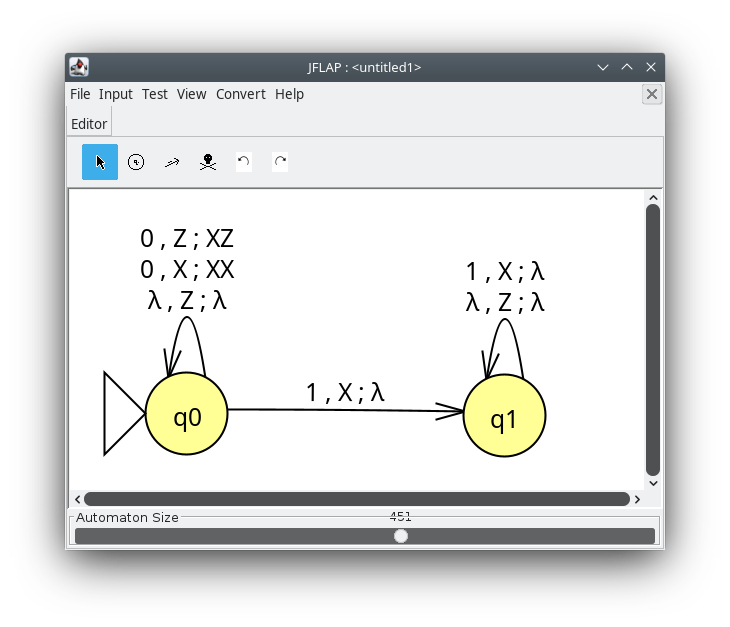
\includegraphics[scale=0.32]{Prácticas/Pila - Pila vacía}
	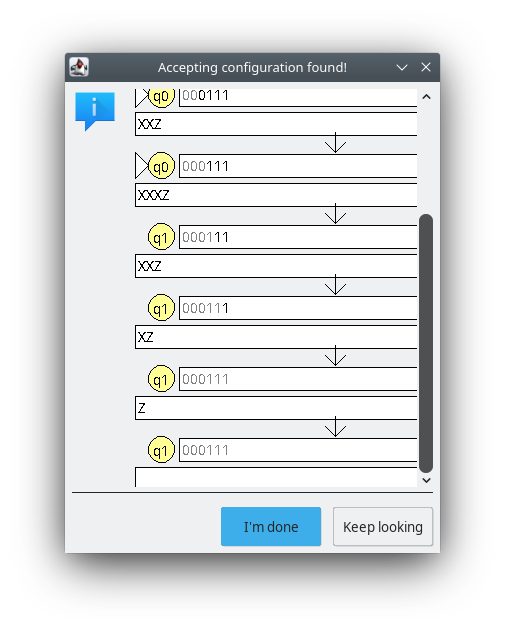
\includegraphics[scale=0.32]{Prácticas/Pila - Pila vacía ejecución}
\end{center}
\caption{Autómata con pila funcionado con el criterio de pila vacía.}
\end{figure}

El problema que tiene este autómata es que no acepta cadenas nulas al usar el criterio de estados finales.
Queremos que este ocmportamiento funcione porque el autómate acepta cadenas con tantos ceros como unos, por lo que la cadena vacía debe ser correcta (ningún cero y ningún uno).
Vamos a modificarlo y comprobar que acepta cadenas vacías:

\begin{figure}[h!]
\begin{center}
	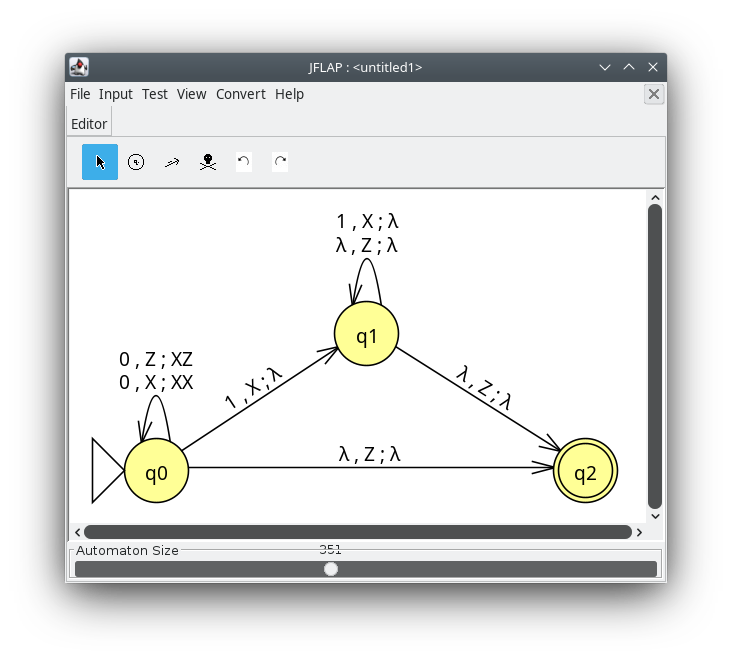
\includegraphics[scale=0.32]{Prácticas/Pila - Estados finales}
	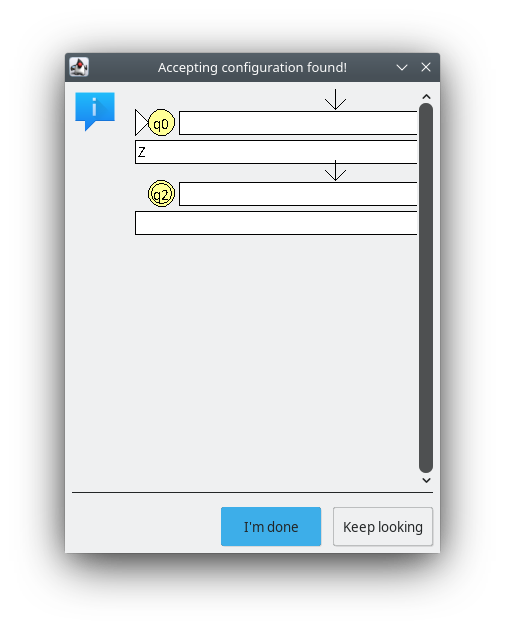
\includegraphics[scale=0.32]{Prácticas/Pila - Estados finales ejecución}
\end{center}
\caption{Autómata con pila funcionado con el criterio de estados finales.}
\end{figure}
